\begin{figure}[H]
\centering
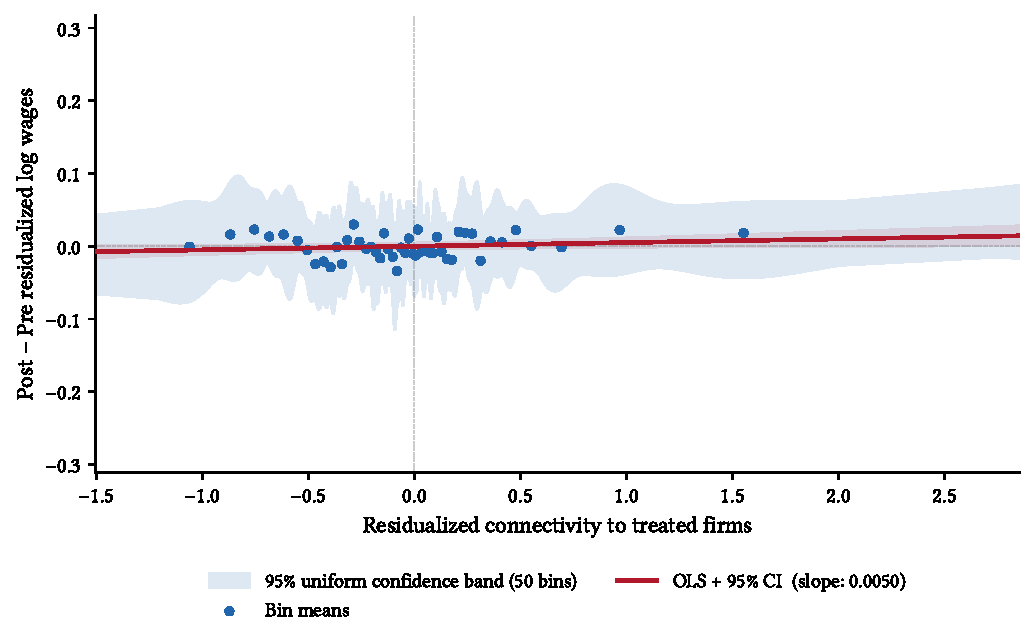
\includegraphics[width=0.75\textwidth]{linearity_fig3_binsreg.pdf}
\caption{Nonparametric Shape of the Connectivity--Wage Relationship}
\label{fig:linearity_binsreg}
\begin{minipage}{0.75\textwidth}
    \vspace{0.3em}
    \footnotesize
    \textit{Notes:} This figure plots the residualized dose--response relationship between pre-treatment connectivity and the post-minus-pre change in residualized log wages. The $x$-axis is the pre-period average of residualized connectivity to treated firms ($\tilde{c}_i$); the $y$-axis is the firm-level difference-in-differences in residualized log wages. Both variables are residualized on industry $\times$ year, negotiation-month $\times$ year, microregion $\times$ year, and baseline wage, size, and flows-per-worker quartile $\times$ year fixed effects; the outcome additionally absorbs firm fixed effects. Dots and the shaded band are, respectively, the bin-mean estimates and the 95\% uniform confidence band from a binscatter with 50 bins \citep{Cattaneo2024}. The solid red line and shaded band are the OLS fit and its 95\% confidence interval. The $p$-value reported in the upper-right corner is from the sup-norm specification test of \citet{Cattaneo2024}, which tests the null hypothesis that the conditional mean $E[y_i \mid x_i]$ is a global linear polynomial; the test fails to reject linearity ($p = 0.468$).
\end{minipage}
\end{figure}
